\documentclass{vgtc}                 % final submission%

\ifpdf%                                % if we use pdflatex
  \pdfoutput=1\relax                   % create PDFs from pdfLaTeX
  \pdfcompresslevel=9                  % PDF Compression
  \pdfoptionpdfminorversion=7          % create PDF 1.7
  \ExecuteOptions{pdftex}
  \usepackage{graphicx}                % allow us to embed graphics files
  \DeclareGraphicsExtensions{.pdf,.png,.jpg,.jpeg} % for pdflatex we expect .pdf, .png, or .jpg files
\else%                                 % else we use pure latex
  \ExecuteOptions{dvips}
  \usepackage{graphicx}                % allow us to embed graphics files
  \DeclareGraphicsExtensions{.eps}     % for pure latex we expect eps files
\fi%

%% it is recomended to use ``\autoref{sec:bla}'' instead of ``Fig.~\ref{sec:bla}''
\graphicspath{{figures/}{pictures/}{images/}{./}} % where to search for the images

\usepackage{microtype}                 % use micro-typography (slightly more compact, better to read)
\PassOptionsToPackage{warn}{textcomp}  % to address font issues with \textrightarrow
\usepackage{textcomp}                  % use better special symbols
\usepackage{mathptmx}                  % use matching math font
\usepackage{times}                     % we use Times as the main font
\renewcommand*\ttdefault{txtt}         % a nicer typewriter font
\usepackage{cite}                      % needed to automatically sort the references
\usepackage{tabu}                      % only used for the table example
\usepackage{booktabs}                  % only used for the table example
%% We encourage the use of mathptmx for consistent usage of times font
%% throughout the proceedings. However, if you encounter conflicts
%% with other math-related packages, you may want to disable it.


%% If you are submitting a paper to a conference for review with a double
%% blind reviewing process, please replace the value ``0'' below with your
%% OnlineID. Otherwise, you may safely leave it at ``0''.
\onlineid{0}

%% declare the category of your paper, only shown in review mode
\vgtccategory{Research}

%% allow for this line if you want the electronic option to work properly
\vgtcinsertpkg

%% In preprint mode you may define your own headline. If not, the default IEEE copyright message will appear in preprint mode.
%\preprinttext{To appear in an IEEE VGTC sponsored conference.}

%% This adds a link to the version of the paper on IEEEXplore
%% Uncomment this line when you produce a preprint version of the article 
%% after the article receives a DOI for the paper from IEEE
%\ieeedoi{xx.xxxx/TVCG.201x.xxxxxxx}


%% Paper title.

\title{Poverty, Income, and COVID-19 in New York City}

%% This is how authors are specified in the conference style

%% Author and Affiliation (single author).
%%\author{Roy G. Biv\thanks{e-mail: roy.g.biv@aol.com}}
%%\affiliation{\scriptsize Allied Widgets Research}

%% Author and Affiliation (multiple authors with single affiliations).
%%\author{Roy G. Biv\thanks{e-mail: roy.g.biv@aol.com} %
%%\and Ed Grimley\thanks{e-mail:ed.grimley@aol.com} %
%%\and Martha Stewart\thanks{e-mail:martha.stewart@marthastewart.com}}
%%\affiliation{\scriptsize Martha Stewart Enterprises \\ Microsoft Research}

%% Author and Affiliation (multiple authors with multiple affiliations)
\author{Irene Zhang\thanks{e-mail: yachun.zhang21@myhunter.cuny.edu}}

%% A teaser figure can be included as follows
\teaser{
  \centering
  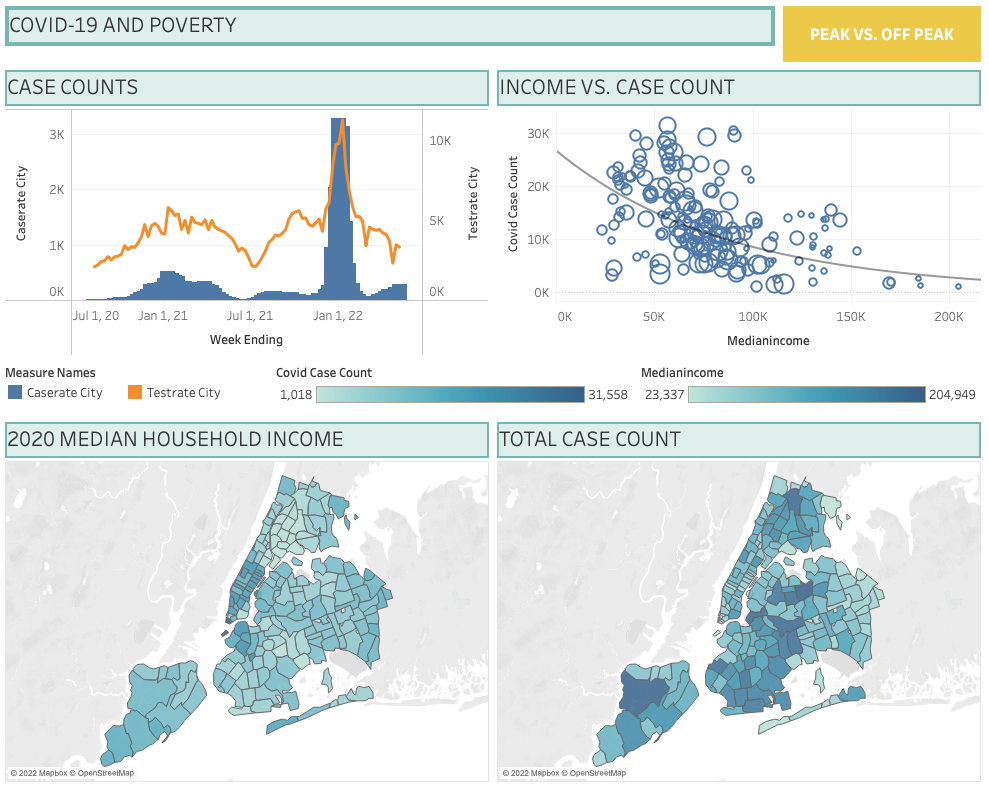
\includegraphics[width=\linewidth]{Dashboard1}
  \caption{Project Dashboard 1.}
  \label{fig:teaser}
}
%% Abstract section.
\abstract{The purpose of this project is to determine the correlation between the COVID-19 pandemic and economic inequalities in New York City. Although the phrase ``COVID-19 does not discriminate" is repeated on various occasions, the disease affects economically disadvantaged people disproportionately, reinforcing and exacerbating the economic inequalities in society through lack of access to resources. The COVID-19 pandemic increases concerns centering around lack of access to safe housing, food, and medical resources, which targets the less privileged group in society. This project studies the relationship between the number of positive cases of coronavirus and average rent in NYC from early 2020 to Spring 2022. Initial results show that the cases in poorer neighborhoods grow faster than in wealthier neighborhoods. 

%
} % end of abstract

%% ACM Computing Classification System (CCS). 
%% See <http://www.acm.org/about/class> for details.
%% We recommend the 2012 system <http://www.acm.org/about/class/class/2012>
%% For the 2012 system use the ``\CCScatTwelve'' which command takes four arguments.
%% The 1998 system <http://www.acm.org/about/class/class/2012> is still possible
%% For the 1998 system use the ``\CCScat'' which command takes four arguments.
%% In both cases the last two arguments (1998) or last three (2012) can be empty.

\CCScatlist{
  \CCScatTwelve{COVID-19 pandemic, modified ZIP Code Tabulation Areas (MODZCTA), poverty threshold, visualization.}{}{}{}
}
%\CCScatlist{
  %\CCScat{H.5.2}{User Interfaces}{User Interfaces}{Graphical user interfaces (GUI)}{};
  %\CCScat{H.5.m}{Information Interfaces and Presentation}{Miscellaneous}{}{}
%}

%% Copyright space is enabled by default as required by guidelines.
%% It is disabled by the 'review' option or via the following command:
% \nocopyrightspace

%%%%%%%%%%%%%%%%%%%%%%%%%%%%%%%%%%%%%%%%%%%%%%%%%%%%%%%%%%%%%%%%
%%%%%%%%%%%%%%%%%%%%%% START OF THE PAPER %%%%%%%%%%%%%%%%%%%%%%
%%%%%%%%%%%%%%%%%%%%%%%%%%%%%%%%%%%%%%%%%%%%%%%%%%%%%%%%%%%%%%%%%

\begin{document}

%% The ``\maketitle'' command must be the first command after the
%% ``\begin{document}'' command. It prepares and prints the title block.

%% the only exception to this rule is the \firstsection command
\firstsection{Introduction}

\maketitle

%% \section{Introduction} %for journal use above \firstsection{..} instead
The project will focus on the relationship between the cases of coronavirus and the economic factors in New York City. Since the beginning of 2020, the COVID-19 pandemic has brought both positive and negative changes to society, influencing over 70 million people. In the city of New York, these changes hit hard on people who are less privileged and completely altered their way of living. This project will look into the average rent in New York City before and after the COVID-19 pandemic and compare it to case rates in each neighborhood, analyzing the connections between the spread of virus and the economic advantages. 

\section{Prerequisites}

The project works with publicly accessible data sources, details will be provided in the bibliography section. The project also requires the 2022.1 version of Tableau Desktop. Visualization of case rates trend and average rent trend will be created by Tableau to analyze the correlation of poverty and spread of COVID-19.

\section{Methodology}

The methodology in this project includes two parts: pre-processing and methods. Pre-processing cleans out any useless data to enhance performance, and the visualizations are made following steps in methods.

\vspace{2mm}
\noindent Live animations are available here :

\vspace{1mm}
\noindent\url{https://public.tableau.com/views/PovertyIncomeandCOVID-19inNewYorkCity/Dashboard1?:language=en-US&:display_count=n&:origin=viz_share_link}

\subsection{Pre-processing}

A preliminary processing of data is done at first in order to prepare the data sets for primary processing and further analysis. Methods for data pre-processing include data cleaning, data integration, data reduction, and data transformation. During the data selection period, the focus was on the completeness and inclusiveness on topics for each data sets, i.e., the complete list of daily case rates by zip-code is chosen over list of monthly case rates by boroughs. Both Excel and Python MySQL were used to reorganize data sets. The data file containing case rates by MODZCTA contains columns such as ``CASERATE\textunderscore 10001". Such column names are altered by eliminating ``CASERATE\textunderscore" to keep only the clean zip-code. The original data set is up to date, which is then cut short to fit the narrative of the research time frame. Similar actions are performed on the median income data set to clean up column names and unwanted areas. 

\subsection{Methods}

The visualizations are created with Tableau. After importing the first data source of case rate by MODZCTA, a new data set of median income data is connected with a common factor of zip-code. 

\begin{figure}[tb]
 \centering % avoid the use of \begin{center}...\end{center} and use \centering instead (more compact)
 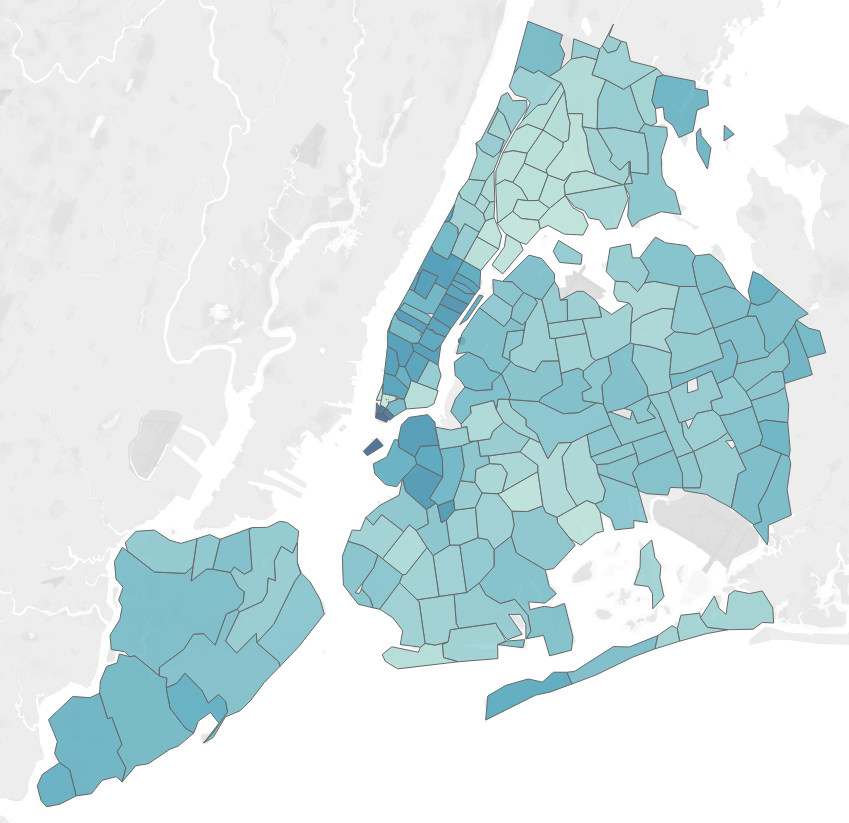
\includegraphics[width=\columnwidth]{income-choropleth.png}
 \caption{A visualization of the current NYC median household income.}
 \label{fig:sample}
\end{figure}

\begin{figure}[tb]
 \centering % avoid the use of \begin{center}...\end{center} and use \centering instead (more compact)
 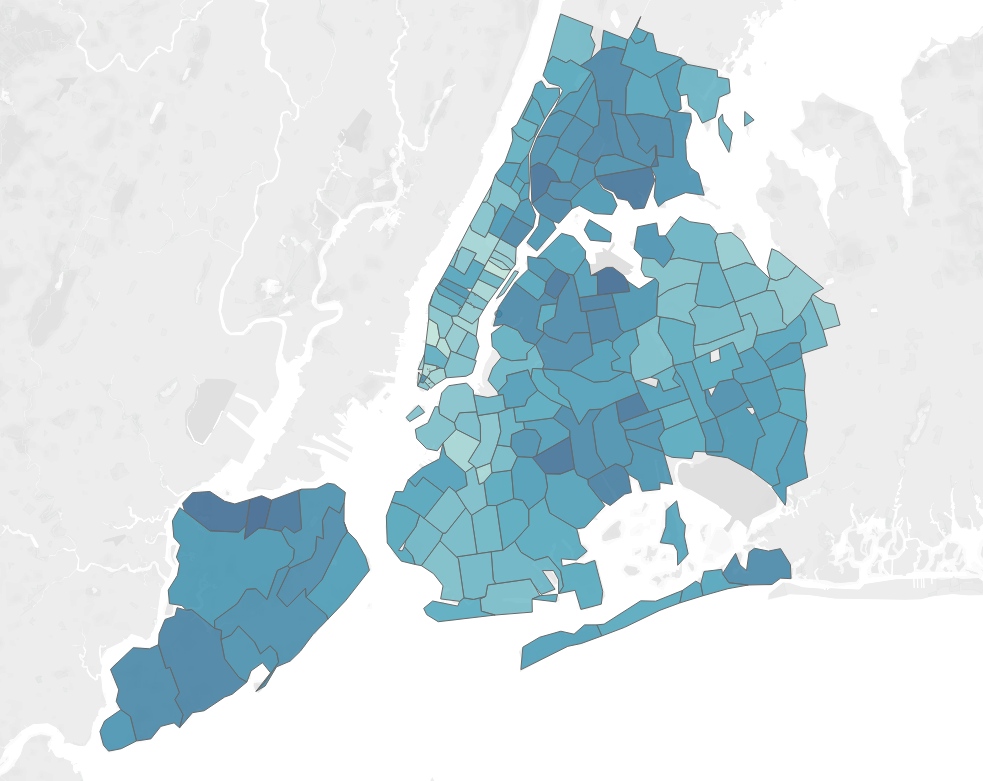
\includegraphics[width=\columnwidth]{Jan22.png}
 \caption{A visualization of the NYC case rate map in January 2022.}
 \label{fig:sample}
\end{figure}

\begin{figure}[tb]
 \centering % avoid the use of \begin{center}...\end{center} and use \centering instead (more compact)
 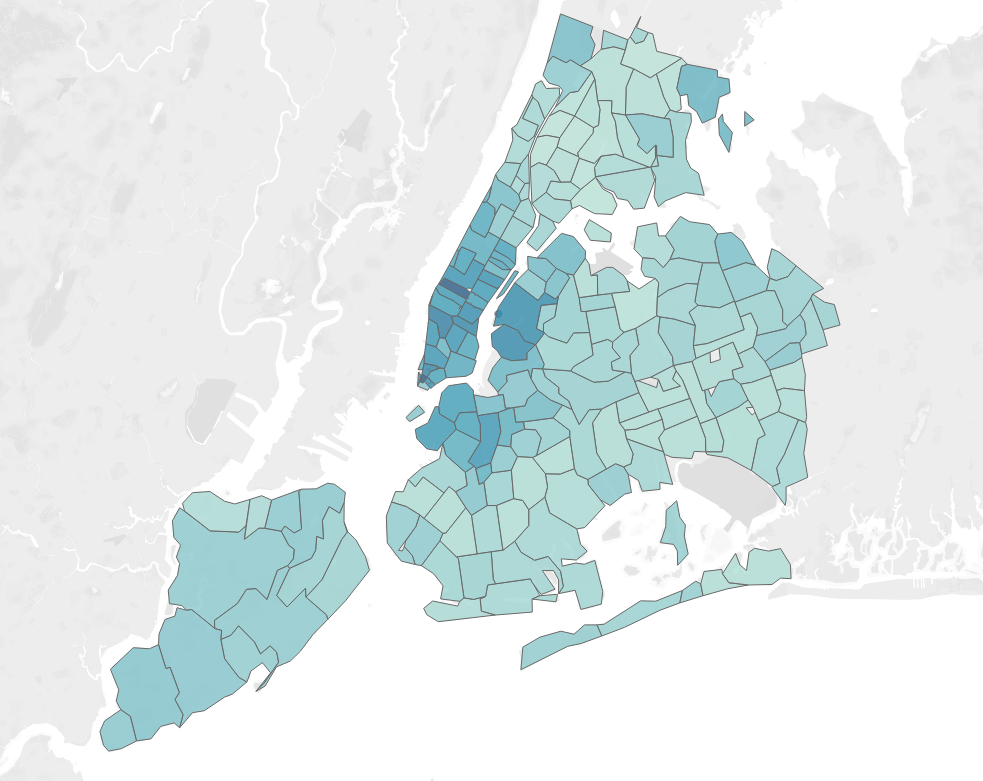
\includegraphics[width=\columnwidth]{Apr22.png}
 \caption{A visualization of the NYC case rate in April 2022.}
 \label{fig:sample}
\end{figure}

\section{initial results}
Figure 2 is a choropleth map showing the 2020 median household income in NYC. Wealth was more concentrated in most parts of Manhattan and downtown Brooklyn. Figure 4 is the case rate in NYC on April 2nd, 2022 when positive cases are slowing down while Figure 3 shows the case rate on the week ending on January 1st, 2022 when the Omicron variant peaked in NYC. In both Figures 3 and 4, the density of color represents the case rates per 100,000 people, the darkest being the most severe. Figure 3 confirmed my hypothesis of the high case rates in underprivileged neighborhoods such as Melrose, New York (zip-code 10451) where its 2020 median income is around \$32,589, almost half of the New York City median of \$67,046. In April 2022, the growth of case rates starts to slow down. One thing I notice about Figure 4 is that this map looks similar to the average income choropleth map of NYC. Neighborhoods with higher COVID-19 case rates are also neighborhoods with higher median incomes when the pandemic is off-peak. One explanation is that the rising number of people returning to the office and tourists visiting the city leads to the increase in case rates in downtown and midtown Manhattan.

\section{further analysis}{
To further analyze the relationship between economic inequalities and the COVID-19 pandemic, figure 5 shows a scatter plot of the median income and current total case count in NYC with the best fit line. As shown in the graph, income and case count has a weak negative correlation where R-Squared equals 0.300591. This partially supports the original hypothesis that income inequality does affect people differently during the pandemic, however, such correlation isn't strong enough to draw a conclusion between the two events. Possible causes include different levels of access to safe housing, nutritious food, and medical support. 
}

\begin{figure}[tb]
 \centering % avoid the use of \begin{center}...\end{center} and use \centering instead (more compact)
 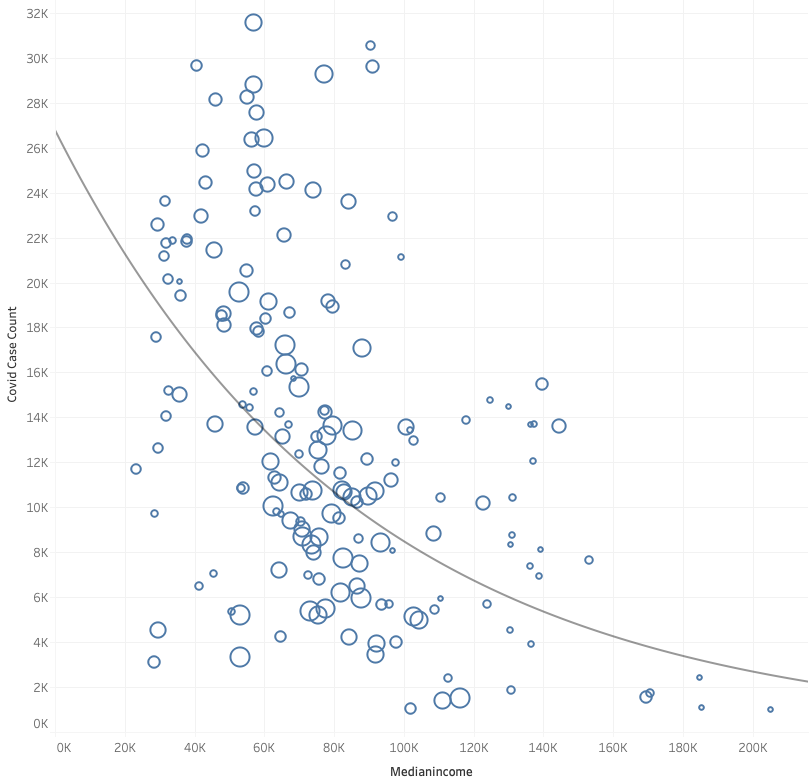
\includegraphics[width=\columnwidth]{incomevscase.png}
 \caption{A scatter plot of median income and case counts.}
 \label{fig:sample}
\end{figure}

\section{limitation and challenges}{
One of the major challenges of this project was the cleaning and connecting process of data sets. For both case rate and test rate data sets, I first transposed the entire data sets to get zip-codes in a column so that it can be used to join two data sets. Then I encountered the error where zip-code columns in two data sets were different in data type. This was fixed by changing one of them into string type. Another issue I saw was while creating the scatter plot for income and case count, the plots showed a weak pattern, and the best fit line did not suggest a strong relationship. This led to further analysis of the pattern.  
}

%% if specified like this the section will be committed in review mode
\section{future work}{
If given more time, this project can be polished for a better interactive dashboard which connects each zip code to its corresponding case count line graph. 
}

\section{Datasets}
\noindent\url{https://github.com/izhang024/Poverty-Income-and-COVID-19-in-NYC/tree/main}

% %% if specified like this the section will be omitted in review mode
\acknowledgements{
This project was supervised by Professor Oyewole Oyekoya, as an Advanced Visualization project at Hunter College, Spring 2022.
}

\end{document}
